\documentclass[]{article}

%opening
%\usepackage{fullpage}
\usepackage{hyperref}
\usepackage[english]{babel}
\usepackage[utf8]{inputenc}
\usepackage{graphicx}
%\usepackage[backend=biber]{biblatex}
%\usepackage{booktabs}
%\usepackage{amsmath}
%\usepackage{listings}
\graphicspath{{img/}}
%\usepackage{caption}
%\usepackage{subcaption}
%\bibliography{references}
\title{Biometrics Systems Concepts:\\ 2D + 3D face recognition}
\author{Tom Decroos\\r0297757}
\begin{document}
\maketitle
\begin{abstract}
This report discusses the implementation of a face recognition system that makes use of 2D and 3D face representations. First, three relevant papers are discussed: a paper about using eigenfaces for facial recognition, a paper about using local binary patterns and a paper about combining 2D and 3D face recognition. Next, we describe the implementation of our face recognition system. Our implementation uses methods that are heavily based on the three papers we read. Finally, experiments are performed for 2D face recognition, 3D face recognition and the combination of 2D and 3D face recognition.
\end{abstract}

\section{Literature study}
We discuss three relevant papers about face recognition systems. The first paper provides a holistic approach for recognizing faces. The used method is eigenfaces. The second paper provides a feature based approach. The used method is local binary patterns.
%The third paper discusses the fusion of 2D and 3D face recognition. It reports on a large experimental study on multimodal face recognition.
For each paper, a small summary is provided. Afterwards, possible advantages and disadvantages of both approaches are discussed. We focus in our summaries and discussion mostly on the parts of the papers that are relevant for this report.

\subsection{Holistic approach: eigenfaces}
The paper we read for recognizing faces with a holistic approach is `Use of depth and colour eigenfaces for face recognition' by F. Tsalakanidou, D.Tzovaras and M.G. Strintzis \cite{tsalakanidou2003use}.
%\paragraph{Summary}
This paper first discusses the extraction of depth maps. Most face recognition systems are based on the evaluation of 2D-intensity or colour im ages. These systems are subject to a variety of errors caused by differences in illumination, head rotation, face pigment or facial expressions. Biometric features from 3D measurements are expected to perform well, due to their relative independence from these differences. One way of exploiting the 3D information of the geometric characteristics of a human face is by building a depth map. The depth map of a face is a function giving for each pixel of an image the distance to the camera. Such a depth map can be extracted from a set of 3D coordinates of points using the z-buffer algorithm.

Next, the classification method is discussed. The paper proposes a powerful global approach (PCA) in which the whole image (colour or depth map) serves as a feature vector and the variability of the face is modelled by analyzing its statistical properties using a large set of faces. PCA is a well-known, widely and successfully used method. The application of PCA for face recognition is very simple: PCA is performed in a well-defined set of images of human faces and a set of principal components is obtained. These principal components are called eigenfaces. Every face in the database can then be represented as a vector of weights. The weights are obtained by projecting the image of the face on the eigenfaces. Identification of a new test image is then done by locating the image in the database whose weights have the smallest euclidean distance from the weights of the test image. The authors of the paper observed experimentally that the accuracy of this approach quickly degrades if there are changes in scale. This can be explained by the low correlation between face images at different scales. Hence, to successfully apply this approach, all faces in the database must be uniformly scaled.

This approach can only be applied on single channel signals such as a depth map or a grayscale image. In case of face recognition from full colour images, this approach is applied to each component of the colour signal. The PCA algorithm is performed for training sets of each component. When a new image needs to be recognized, its projection to the subspace of each component is computed. The image is then assigned to the class that results in the smallest product of the euclidean distances of each component. This combination approach based on the product of the euclidean distances of each component can also be used to combine a colour and a depth map for 2D + 3D face recognition.

Finally, the eigenfaces approach was evaluated on three representations of faces: colour map, depth map and combination of colour and depth. Experiments were performed on images of 40 people. For each person, there were four colour images and two depth maps available. The training set consisted of two colour images and one depth map for each person. The test set consisted of the remaining two colour images and depth map for each person. The eigenfaces approach achieves a recognition rate of 87.5\% using only colour images, 85\% using depth maps and 97.5\% using the combination. These results show that adding depth information leads to significant gains in recognizing faces.

\subsection{Feature based approach: local binary patterns}
The paper we read for recognizing faces with a feature based approach is `Face Recognition with Local Binary Patterns' by T. Ahonen, A. Hadid and M. Pietikäinen \cite{ahonen2004face}.
The paper first explains the concept of local binary patterns (LBP). The original LBP operator is a powerful means of texture description. The operator labels the pixels of an image by thresholding the 3x3 neighbourhood of each pixel with the center value and considering the result as a binary number (Figure \ref{fig:lbp-explained}). This basic operator can be extended by using neighbourhoods of different sizes and using only uniform patterns.
\begin{figure}
\centering
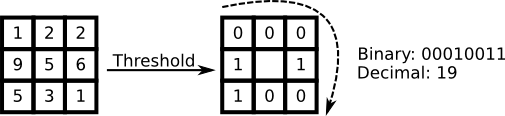
\includegraphics{lbp_explained.png}
\caption{The basic LBP operator.}
\label{fig:lbp-explained}
\end{figure}

The histogram of the labels can then be used as a texture descriptor. This histogram contains information about the distribution of the local micropatterns, such as edges, spots and flat areas, over the whole image. For efficient face representation, one should also retain spatial information. For this purpose, the image is divided into different regions. The histograms of each separate region are then concatenated and form a spatially enhanced histogram. In this histogram, we effectively have a description of the face on three different levels of locality: the labels for the histogram contain information about the patterns on a pixel-level, the labels are summed over a small region to produce information on a regional level and the regional histograms are concatenated to build a global description of the face.

Several possible dissimilarity measures exist for histograms, such as histogram intersection, Log-likelihood statistic and Chi square statistic ($\chi^2$) When the image has been divided into regions, it can be expected that some of the regions contain more useful information than others in terms of distinguishing between people. For example, eyes seem to be an important cue in human face recognition. To take advantage of this, a weight can be set for each region based on the importance of the information it contains. 

The paper used the CSU Face Identification Evaluation System for testing the performance of its proposed algorithm. The results show that $\chi^2$ was the best distance measure between histograms for recognizing faces. They also show that the LBP algorithm is quite robust with respect to its parameters, such as neighbourhood size. Changes in the parameters may cause big differences in the length of the feature vector, but the overall performance is not necessarily affected significantly. When compared to other algorithms such as Eigenfaces, Fisherfaces or Elastic Bunch Graph Matching, the LBP algorithm significantly outperforms them all.

\subsection{Discussion}
Experiments in \cite{chang2005evaluation} suggest that the Eigenfaces approach works best when used on a face space that was generated from a lot of images with diverse conditions (eg. lighting or facial expression). This might be a problem, because our training and test set only consist of five persons each. This means that our face space would be based on only five images. We fear that this face space would incorporate too many specific characteristics of these five images, which would lead to a less accurate result on new images. The LBP algorithm generates features from each image in an independent way, the size of the dataset does not affect its performance. This is a useful characteristic when dealing with small datasets.

It has also been observed experimentally that the performance of the Eigenfaces approach degrades quickly as the scale changes. Intuitively, this is explained by the low correlation between faces and images at different scales. The LBP algorithm considers not only shape, but also texture information to represent face images. That is why we expect the LBP algorithm to be a bit more robust with respect to scale than the Eigenfaces approach.

% eigenfaces need more data
% eigenfaces don't scale well
% sensitive to light
%lbp is independent from other data
%lbp searches for patters, size is less important.
%micro-patterns invariant to monotonic grey scale trasnformation
%\subsection{Fusion of 2D and 3D face recognition}
\section{Methods}
%preprocessing on 2d faces
%splitting colour images in 3 channels

%how depth map was generated, 1.remove outliers 2. grid data

%using LBP algorithm because better than eigenfaces, confirmed in pilot experiments
%combining match scores by multiplying

\section{Experiments}
% already almost perfect score for training set + no real parameters to tune -> lets use full set

% results for 4 channels, colour and colour + depth

% results after preprocessing: 4 channels, colour and colour + depth 
\section{Conclusion}
%\printbibliography
\bibliography{references}
\bibliographystyle{plain}
\end{document}